\documentclass{article}
\usepackage{titlesec}
\usepackage[dotinlabels]{titletoc}
\usepackage[utf8]{inputenc}
\usepackage[russian]{babel}
\usepackage[a4paper, left=1.5cm, right=1.5cm, top=1cm, bottom=1cm]{geometry}
\usepackage[unicode, pdftex]{hyperref}
\setlength\parindent{0pt}
\pagenumbering{gobble}
\usepackage{caption} 
\captionsetup[table]{skip=5pt}
\usepackage{graphicx}
\usepackage{float}

\begin{document}

\begin{minipage}{0.62\textwidth}
    \begin{center}
        Санкт-Петербургский национальный исследовательский университет \\
        информационных технологий, механики и оптики \\
        УЧЕБНЫЙ ЦЕНТР ОБЩЕЙ ФИЗИКИ ФТФ
    \end{center}
\end{minipage}
\hfill
\begin{minipage}{0.38\textwidth}
    \centering
    \begin{figure}[H]
    
\includegraphics[width=\textwidth]{logo.png}
    \end{figure}
\end{minipage}

\rule{\textwidth}{1pt} \\

\begin{minipage}{0.16\textwidth}
        Группа \hrulefill\\
        Студент \hrulefill\\
        Преподаватель \hrulefill
\end{minipage}%
\begin{minipage}{0.25\textwidth}
        K3222\hrulefill\\
        Бевз Т.А.\hrulefill\\
        Соломонов А.И.\hrulefill
\end{minipage}
\hfill
\begin{minipage}{0.47\textwidth}
        К работе допущен \hrulefill\\
        Работа выполнена \hrulefill\\
        Отчёт принят \hrulefill
\end{minipage}
\begin{center}
    \textbf{\huge Рабочий протокол и отчет по \\
    лабораторной работе № 4.09}
\end{center}
\begin{minipage}{1\textwidth}
        \hrulefill\\
        \Large\textbf{Исследование поляризации света (стопа Столетова)}\hrulefill
\end{minipage}
\section{Цель работы}
\begin{enumerate}
     Изучение поляризованного света и определение показателей преломления.
\end{enumerate}

\section{Задачи, решаемые при выполнении работы}
\begin{enumerate}
    \item Измерение фототока при различных углах поворота анализатора.
    \item Расчет косинуса и косинуса в квадрате угла поворота анализатора.
    \item Построение графика зависимости фототока $I$ от $cos^2(\alpha)$.
    \item Измерение фототока интенсивности отраженного и преломленного лучей для p- и s- компонент света при различных углах падения света с помощью стопы Столетова.
    \item Построение графиков зависимостей фототоков интенсивности $i$ от угла падения $\phi$.
    \item Нахождение по графикам угла Брюстера $\phi_{Br}$ и коэффициента преломления стекла $n$.
\end{enumerate}

\section{Объект исследования}
Поляризатор (поляроид) и анализатор (поляроид, стопа Столетова).
\section{Метод экспериментального исследования}
Физический эксперимент.
\section{Рабочие формулы и исходные данные}
\begin{equation}
 tan\phi_{Br}=n_{21} - \textit{Тангенс угла Брюстера.}
 \label{eq:ref1}
\end{equation}
Где $n_{21}$ - показатель преломления второй среды относительно первой.
\begin{equation}
 I=I_{0}cos^2\alpha - \textit{Интенсивность прошедшего света.}
 \label{eq:ref2}
\end{equation}
Где $I_{0}$ - интенсивность падающего на поляризатор света, $\alpha$ - угол поворота анализатора.
\newpage
\section{Измерительные приборы}
\begin{table}[h]
    \centering
    \bgroup
    \def\arraystretch{1.2}
    \begin{tabular}{|c|c|c|c|}
        \hline
        Наименоване & Тип прибора & Используемый диапазон & Погрешность \\
        \hline
        Фоторезистор & Цифровой & $0-200$ мкА. & $0.5$ мкА. \\
        \hline
    \end{tabular}
    \egroup
    \caption{Измерительные приборы} 
\end{table}
\section{Схема установки}
\begin{figure}[h!]
    \begin{center}
    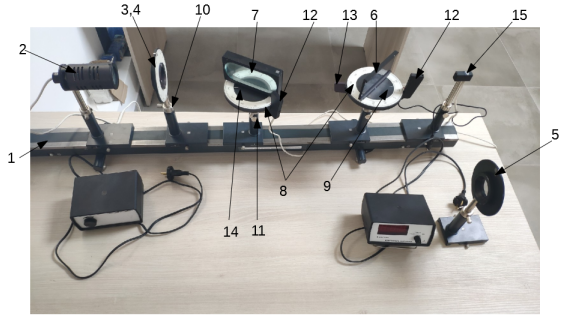
\includegraphics[width=0.6\textwidth]{scheme.png}
    \caption{Рабочая схема исследования поляризации света. 1 - скамья, 2 - источник света, 3 - поляроид, 4 - оправа с лимбом, 5 - анализатор (поляроид), 7 - анализатор (стопа Столетова), 15 - рейтер с фоторезистором.}
    \label{fig:scheme}    
    \end{center}
\end{figure}
\section{Ход работы}
\begin{itemize}
  \item Для обработки результатов лабораторной работы было необходимо отметить показания фототока $I$ проходящего через поляризатор света при различных углах поворота анализатора $\alpha$. Результаты представлены в таблице №2.
  \item На основе полученных данных, для подтверждения закона Малюса был построен график зависимости $I(cos^2\alpha)$. Он подтвердил работу этого закона, однако с небольшими отклонениями значений фототока при одиннаковых значениях $cos^2\alpha$. График представлен на рисунке №2.
  \item Далее были отмечены показатели фототока интенсивности для преломленного и отраженного стопой Столетова лучей s- и p- компонент света при различных углах падения. Результаты представлены в таблице №3.
  \item После этого, были построены график зависимости приломленного и отраженного лучей p-компоненты света от угла падения. Их видно на рисунке №3. А также график зависимости приломленного и отраженного лучей s-компоненты света от угла падения. Их видно на рисунке №4
  \item На основе этих графиков на рисунках №3 и №4 был найден угол Брюстера $\phi_{Br} = 55^\circ$. При таком угле падения, отраженный свет является полностью поляризованным.
  \item Наконец, с помощью найденного угла Брюстера был найден показатель преломления стекла $n = tan\phi_{Br}=1.428$.
\end{itemize}
\newpage
\section{Результаты прямых измерений и их обработки}
\begin{table}[h]
    \centering
    \bgroup
    \def\arraystretch{1.4}
    \begin{tabular}{|c|c|c|c|c|}
        \hline
        № & Угол поворота $\alpha$, $^\circ$ & $cos\alpha$ & $cos^2\alpha$ & $I$, мкА \\ \hline
        $ 1 $ & $ 0 $ & $ 1.00 $ & $ 1.00 $ & $ 7.42 $\\ \hline
        $ 2 $ & $ 10 $ & $ 0.98 $ & $ 0.97 $ & $ 6.93 $\\ \hline
        $ 3 $ & $ 20 $ & $ 0.94 $ & $ 0.88 $ & $ 5.84 $\\ \hline
        $ 4 $ & $ 30 $ & $ 0.87 $ & $ 0.75 $ & $ 4.69 $\\ \hline
        $ 5 $ & $ 40 $ & $ 0.77 $ & $ 0.59 $ & $ 3.46 $\\ \hline
        $ 6 $ & $ 50 $ & $ 0.64 $ & $ 0.41 $ & $ 2.26 $\\ \hline
        $ 7 $ & $ 60 $ & $ 0.50 $ & $ 0.25 $ & $ 1.25 $\\ \hline
        $ 8 $ & $ 70 $ & $ 0.34 $ & $ 0.12 $ & $ 0.55 $\\ \hline
        $ 9 $ & $ 80 $ & $ 0.17 $ & $ 0.03 $ & $ 0.23 $\\ \hline
        $ 10 $ & $ 90 $ & $ 0.00 $ & $ 0.00 $ & $ 0.2 $\\ \hline
        $ 11 $ & $ 100 $ & $ -0.17 $ & $ 0.03 $ & $ 0.41 $\\ \hline
        $ 12 $ & $ 110 $ & $ -0.34 $ & $ 0.12 $ & $ 0.96 $\\ \hline
        $ 13 $ & $ 120 $ & $ -0.50 $ & $ 0.25 $ & $ 1.85 $\\ \hline
        $ 14 $ & $ 130 $ & $ -0.64 $ & $ 0.41 $ & $ 3.02 $\\ \hline
        $ 15 $ & $ 140 $ & $ -0.77 $ & $ 0.59 $ & $ 4.35 $\\ \hline
        $ 16 $ & $ 150 $ & $ -0.87 $ & $ 0.75 $ & $ 5.63 $\\ \hline
        $ 17 $ & $ 160 $ & $ -0.94 $ & $ 0.88 $ & $ 6.52 $\\ \hline
        $ 18 $ & $ 170 $ & $ -0.98 $ & $ 0.97 $ & $ 7.06 $\\ \hline
        $ 19 $ & $ 180 $ & $ -1.00 $ & $ 1.00 $ & $ 7.12 $\\ \hline
    \end{tabular}
    \egroup
    \caption{Значения фототока при различных углах поворота анализатора.} 
\end{table}
\newpage
\begin{table}[h]
    \centering
    \bgroup
    \def\arraystretch{1.4}
    \begin{tabular}{|c|c|c|c|c|c|}
        \hline
        № & Угол падения $\phi$, $^\circ$ & Фототок $i^{(p)}_{\textit{пр}}$, мкА & Фототок $i^{(p)}_{\textit{отр}}$, мкА & Фототок $i^{(s)}_{\textit{пр}}$, мкА & Фототок $i^{(s)}_{\textit{отр}}$, мкА\\ \hline
        $1$ & $ 5 $ & $ 9.32 $ & $ 7.75 $ & $ 7.53 $ & $ 6.25 $\\ \hline
        $2$ & $ 10 $ & $ 9.13 $ & $ 7.13 $ & $ 6.64 $ & $ 9.11 $\\ \hline
        $3$ & $ 15 $ & $ 8.63 $ & $ 8.54 $ & $ 6.71 $ & $ 11.23 $\\ \hline
        $4$ & $ 20 $ & $ 8.01 $ & $ 9.11 $ & $ 6.19 $ & $ 11.42 $\\ \hline
        $5$ & $ 25 $ & $ 6.85 $ & $ 9.44 $ & $ 5.48 $ & $ 12.03 $\\ \hline
        $6$ & $ 30 $ & $ 5.43 $ & $ 10.05 $ & $ 4.33 $ & $ 13.13 $\\ \hline
        $7$ & $ 35 $ & $ 3.98 $ & $ 11.50 $ & $ 3.70 $ & $ 14.09 $\\ \hline
        $8$ & $ 40 $ & $ 2.42 $ & $ 13.28 $ & $ 2.47 $ & $ 14.39 $\\ \hline
        $9$ & $ 45 $ & $ 0.95 $ & $ 14.72 $ & $ 2.06 $ & $ 15.58 $\\ \hline
        $10$ & $ 50 $ & $ 0.19 $ & $ 16.87 $ & $ 1.36 $ & $ 17.61 $\\ \hline
        $11$ & $ 55 $ & $ 0.14 $ & $ 17.60 $ & $ 0.86 $ & $ 18.88 $\\ \hline
        $12$ & $ 60 $ & $ 1.37 $ & $ 15.26 $ & $ 1.01 $ & $ 18.79 $\\ \hline
        $13$ & $ 65 $ & $ 4.72 $ & $ 11.91 $ & $ 1.25 $ & $ 18.53 $\\ \hline
        $14$ & $ 70 $ & $ 10.26 $ & $ 5.82 $ & $ 1.34 $ & $ 18.37 $\\ \hline
        $15$ & $ 75 $ & $ 12.32 $ & $ 0.76 $ & $ 1.41 $ & $ 18.12 $\\ \hline
    \end{tabular}
    \egroup
    \caption{Значения фототоков для различных лучей при разных углах падения света.} 
\end{table}
\newpage
\section{Графики}
\begin{figure}[h!]
    \begin{center}
    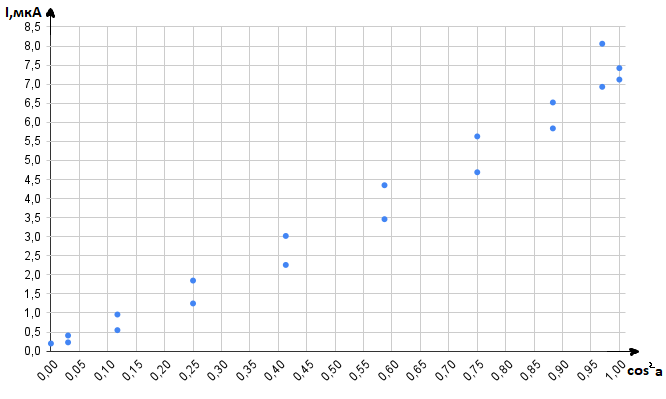
\includegraphics[scale=0.7]{chart1.png}
    \caption{Зависимость фототока от квадрата косинуса угла поворота анализатора $I$ от $cos^2\alpha$}
    \label{fig:graphUfromI}    
    \end{center}
\end{figure}
\begin{figure}[h!]
    \begin{center}
    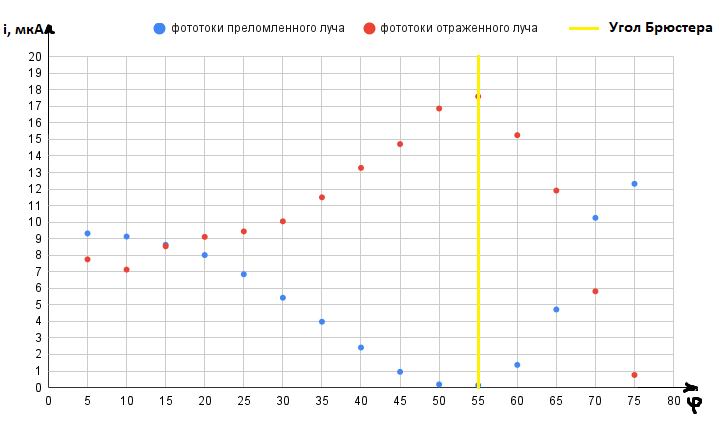
\includegraphics[scale=0.7]{chart2.png}
    \caption{Зависимость фототоков от угла падения света для p-компоненты $i$ от $\phi$}
    \label{fig:graphUfromI}    
    \end{center}
\end{figure}
\begin{figure}[h!]
    \begin{center}
    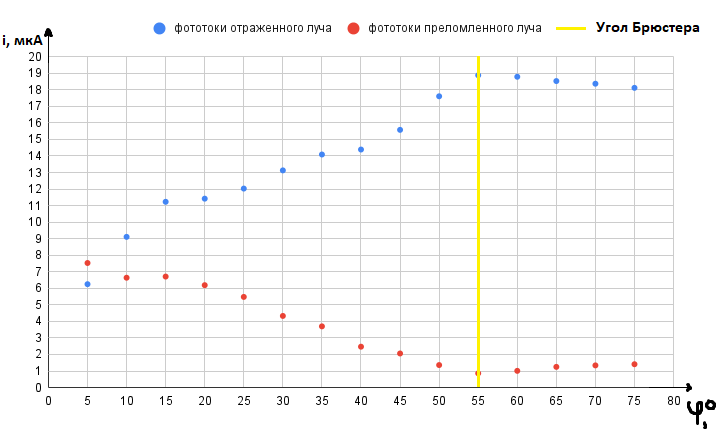
\includegraphics[scale=0.7]{chart3.png}
    \caption{Зависимость фототоков от угла падения света для s-компоненты $i$ от $\phi$}
    \label{fig:graphUfromI}    
    \end{center}
\end{figure}
\newpage
\section{Окончательные результаты}
\begin{enumerate}
    \item Угол Брюстера: $\phi_{Br} = 55^\circ$  
    \item Показатель преломления стекла относительно воздуха: Табличное значение $n_{\textit{т}} = 1.52$; Экспериментальное $n_{\textit{э}} = 1.428$ (Расхождение 6.4$\%$);
\end{enumerate}
\newpage
\section{Вывод}
Входе работы была исследована поляризация света. Экспериментальным путём
подтвердили закон Малюса: при одинаковых косинусах угла поворота значения фототока различались незначительно. Небольшие отклонения, скорее всего, связаны с человеческим фактором и погрешностью оборудования. Был найден угол Брюстера для стекла с помощью исследования фототоков интенсивности преломленного
и отраженного лучей двух компонент света через стопу Столетова. Он составил $55^\circ$. По этому углу был найден показатель преломления стекла, равный 1,428. От табличных найденные значения отличаются незначительно,
что подтверждает достоверность формул.
\end{document}
